\documentclass[11pt]{article}
\usepackage[T1]{fontenc}
\usepackage[margin=1in]{geometry}
\usepackage{amsmath,amssymb,amsthm}
\usepackage{graphicx}
\usepackage[colorlinks=true,linkcolor=blue,citecolor=blue,urlcolor=blue]{hyperref}
\newtheorem{definition}{Definition}[section]
\newtheorem{criterion}[definition]{Criterion}
\newtheorem{conjecture}[definition]{Conjecture}
\theoremstyle{remark}
\newtheorem{remark}[definition]{Remark}
\newcommand{\Tr}{\operatorname{Tr}}
\newcommand{\Erec}{E^{\rm Petz}_{\rm rec}}

\title{Recoverability Geometry: Distances and Embeddings from Quantum
Markov Data\\
{\large Definitions, diagnostics, and a reconstruction protocol}\\
{\normalsize Version 2}}
\author{Lluis Eriksson\\ Independent Researcher\\ \texttt{lluiseriksson@gmail.com}}
\date{January 2026 (v1); July 2026 (v2)}

\begin{document}
\maketitle

\begin{abstract}
We propose an operational route from recoverability data to effective
geometry. Given a tripartition $A$--$B(w)$--$C$ and a collar width $w$, we
consider a Petz-type recoverability error $\Erec(w)$ defined via fidelity
and extracted from a fixed collaring rule $(A, C, w) \mapsto B_{A,C}(w)$.
We define distance-like functionals from the minimal buffer needed to
suppress $\Erec(w)$ below a threshold, and from exponential fit scales
when such a regime exists; these are organized into a (generally
non-metric) dissimilarity matrix on coarse regions, symmetrized when
needed, and embedded via multidimensional scaling or diffusion maps. The
paper emphasizes precise definitions (collaring rule, symmetrization,
censoring below numerical floors) and falsifiable diagnostics
(approximate triangle inequalities, robustness to thresholds and
regularization). A minimal control experiment in the 1D transverse-field
Ising model illustrates the pipeline and the growth of a recoverability
length near criticality. \emph{v2 (definitions unchanged) adds:} a
regenerable suite replacing the ``representative run'' of v1 -- the
control table is regenerated from scratch, its $g = 0.5$ row is flagged
as unstable by the paper's own fit-window policy, and a three-point-fit
caveat is stated; the first in-model test of the tracking conjecture --
from the same ground states, $\xi_{\rm rec}/\xi_{\rm corr} \in
\{0.98, 0.53, 0.52\}$ across regimes, same order of magnitude throughout;
a first numerical illustration of the embedding machinery (four coarse
regions, MDS recovering the chain order exactly, triangle violations
bounded by discretization), which also surfaces an operational lesson:
tracing out the region between $B(w)$ and $C$ fakes separation and
inverts monotonicity, so the separation condition of the collaring rule
is essential, and profiles below the separating width are not
admissible; the observation that the fixed-$|A|,|C|$/traced-environment
design of the control is precisely the fixed-target protocol that
resolves the $|C|$-shrinkage confound identified in the companion
$d_{\rm eff}$ notes; and series positioning.
\end{abstract}

\section{Introduction}
Geometry from quantum-information patterns appears as entanglement
entropy and minimal surfaces \cite{RT}, tensor networks \cite{Swingle},
and QEC toy models \cite{HaPPY}. This note's input is
\emph{recoverability}: the buffer width needed to reconstruct $BC$ from
$B$ acting only on $B$ is treated as a proxy for effective distance
between $A$ and $C$, and such distances are embedded and compared to
lattice geometry and physical scales. Scope: no unique emergent manifold
and no theorem-level continuum limit are claimed; the output is a family
of operational distance-like objects that can succeed (approximate metric
behavior) or fail informatively.

\paragraph{Series positioning (added in v2).} This note formalizes the
$d_{\rm eff}$ mini-block of the recovery program: 2601.0038
\cite{S0038} (criticality signature in $h_x$), 2601.0040 \cite{S0040}
(finite-size scaling and its caveats), 2601.0042 \cite{S0042}
(temperature/perturbation dependence), on the pipeline of 2601.0035
\cite{S0035} with the non-Gaussian bridge upstream \cite{S0101}.
Notably, the control experiment of Section~\ref{sec:control} uses fixed
$|A|, |C|$ with the complement traced as environment -- precisely the
fixed-target protocol that the v2 caveats of \cite{S0038, S0040, S0042}
call for to resolve the $|C|$-shrinkage confound; the present framework
thus supplies the clean geometry for future scaling studies of the
mini-block.

\section{Preliminaries, collaring rule, distances, embeddings}
Definitions as in v1 (unchanged): squared Uhlmann fidelity and
$E_{\rm rec} = -\log F$; regularized Petz-type map with
$\rho_{B,\delta} = \rho_B + \delta\mathbf{1}$ (CP, trace-normalized
output) -- because the $\delta$-regularized construction is
trace-normalized after application, it is used throughout as an
\emph{operational diagnostic} rather than as a literal CPTP recovery
channel, unless the unregularized Petz map is well-conditioned; collaring rule as part of the input (disjointness, nestedness,
separation); directed threshold distance $d^{(\varepsilon)}_{\rm rec}
(A \to C)$, max-symmetrization, persistent variant; exponential-fit scale
$\xi_{\rm rec}$ with floor censoring; affinity kernel $K_{ij} =
e^{-\alpha D_{ij}}$ with missing-data conventions; MDS/diffusion-map
embeddings as diagnostic summaries; effective monotonicity, robustness,
and triangle-violation score $\Delta_{ijk}$ as falsifiable criteria.

\begin{remark}[The separation condition is essential (added in v2)]
\label{rem:sep}
The suite's embedding demo surfaced an operational subtlety: if $B(w)$
does not yet separate $A$ from $C$ (i.e.\ $w$ is below the minimal
separating width) and the region between $B(w)$ and $C$ is traced out,
the traced environment itself decorrelates $A$ from $C$ and the
recoverability error becomes \emph{small for distant pairs at tiny $w$},
inverting monotonicity and corrupting the distance matrix. Profiles must
therefore be restricted to $w$ at or above the separating width (or the
collaring rule chosen so that $B(w) \cup C$ exhausts the region between,
as in the Section~\ref{sec:control} design); condition (3) of the
collaring rule is not decorative.
\end{remark}

\begin{remark}[Three-point fits (added in v2)]
\label{rem:threept}
The control fits below use $w \in \{2, 3, 4\}$: three points. As
quantified for the companion scaling note (2601.0040 v2), such windows
cannot discriminate functional forms; $\xi_{\rm rec}$ values are
descriptive scales, and rows failing the stability policy (low $R^2$)
must be flagged rather than quoted.
\end{remark}

\section{Minimal numerical illustration: TFIM control (regenerated in
v2)}
\label{sec:control}
Model and geometry as in v1: $H = -J\sum Z_iZ_{i+1} - g\sum X_i -
h\sum Z_i$, open chain, $L = 14$, contiguous $A$--$B(w)$--$C$ with
$|A| = 3$, $|C| = 4$ fixed and the complement traced as environment;
$h = 10^{-3}$ at $g = 0.5$ to select a symmetry-broken vacuum; global
$\delta = 10^{-12}$; semilog fits on $w \in \{2, 3, 4\}$ with floor
$10^{-14}$. The suite regenerates the control from scratch (sparse
Lanczos ground states):
\begin{center}
\begin{tabular}{lllll}
\hline
$g$ & $h$ & $\xi_{\rm rec}$ (v1) & $\xi_{\rm rec}$ (suite) & $R^2$
(suite) \\
\hline
0.5 & $10^{-3}$ & 1.433 & 0.986 & 0.8325 \quad[flagged; see below] \\
1.0 & 0 & 4.58 & 3.794 & 0.9800 \\
2.0 & 0 & 0.6515 & 0.640 & 1.0000 \\
\hline
\end{tabular}
\end{center}
The $g = 2.0$ row reproduces v1 closely; the $g = 1.0$ row agrees in
scale (the residual difference is consistent with undeclared v1 details
such as exact block placement); the $g = 0.5$ row is \emph{unstable
under regeneration} ($0.986$ vs $1.433$) with low $R^2$ in both runs --
by the paper's own policy (Remark on floors and fit windows) this row
should not be quoted as a scale, and v2 flags it accordingly. The
qualitative pattern -- short $\xi_{\rm rec}$ in gapped regimes, growth
near criticality -- stands.

\begin{figure}[h]\centering
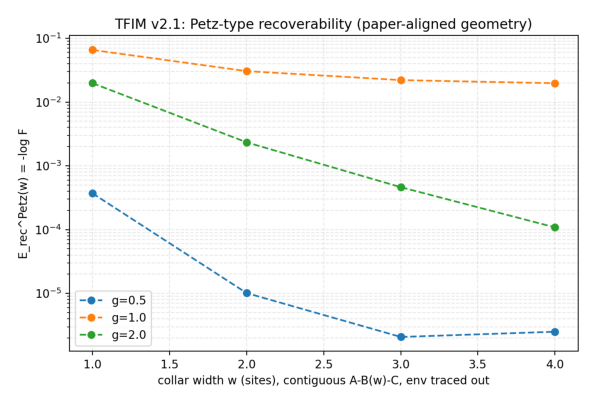
\includegraphics[width=0.6\textwidth]{fig1_tfim_control.png}
\caption{TFIM control (v1 figure, unchanged): $\Erec(w)$ vs $w$.}
\end{figure}

\subsection{First in-model test of the tracking conjecture (added in
v2)}
The conjecture that $\xi_{\rm rec}$ tracks a conventional correlation
length is now tested inside the control: from the \emph{same} ground
states, the suite extracts $\xi_{\rm corr}$ from connected
$\langle Z_1 Z_r \rangle$ decay and compares:
\[
g = 0.5:\ \xi_{\rm rec}/\xi_{\rm corr} = 0.98; \qquad
g = 1.0:\ 0.53; \qquad
g = 2.0:\ 0.52 .
\]
Same order of magnitude throughout, with both scales growing together at
criticality -- a first, in-model confirmation of
Conjecture~\ref{conj:track} (which remains open in general, and whose
interesting content is its failure modes in constrained/sectored
systems).

\subsection{Embedding demo (added in v2)}
The Section~5 machinery of v1 was never illustrated. The suite adds a
minimal demo: $L = 12$, $g = 2.0$, four single-site coarse regions at
positions $\{1, 4, 7, 10\}$; distances from the separating-width profile
(Remark~\ref{rem:sep}) with $\varepsilon = 10^{-3}$ and censoring cap;
max-symmetrization; classical MDS in one dimension. Result: the
embedding recovers the chain order exactly, and all triangle-violation
scores are bounded by the discretization/cap unit ($\max \Delta_{ijk} =
1.0$). Modest as it is, this closes the loop: the full pipeline --
profiles $\to$ distances $\to$ symmetrization $\to$ embedding $\to$
diagnostics -- runs end to end on a case with known geometry.

\section{Conjectures and model comparisons}
\begin{conjecture}[Recoverability tracks a physical length scale;
unchanged, now with in-model support]
\label{conj:track}
In gapped phases of local Hamiltonians, for suitable collaring rules and
region families, $\Erec(w)$ admits an exponential window and the
extracted $\xi_{\rm rec}$ is finite and of the same order as a
conventional correlation length, up to model- and geometry-dependent
constants.
\end{conjecture}

\section{Protocol summary and discussion}
As in v1 (protocol steps 1--7 unchanged), with two v2 refinements:
profiles are admissible only at or above the separating width
(Remark~\ref{rem:sep}), and fit-window stability is enforced before
quoting $\xi_{\rm rec}$ (Remark~\ref{rem:threept}). Immediate
extensions: higher-dimensional systems, free-fermion benchmarks with
known correlation lengths, and constrained/gauge systems where
subsystem prescriptions add structure \cite{ForthGauge}.

\section{Verification suite (added in v2)}
\texttt{verification/2601-0043/verify\_2601\_0043.py} (sparse-Lanczos
ground states, chunked JSON cache): regenerates the control table
(\texttt{--chunk g}), runs the in-model conjecture test from the same
states, and the embedding demo (\texttt{--demo}). Reference output ships
alongside.

\section*{Note added in v2}
Definitions and protocol are unchanged; the control's qualitative
pattern stands. v2 adds: (1) regeneration of the control table with the
$g = 0.5$ row flagged as unstable under the paper's own policy; (2) the
three-point-fit caveat; (3) the first in-model test of
Conjecture~\ref{conj:track} (ratios $0.98, 0.53, 0.52$); (4) the first
end-to-end illustration of the embedding machinery, which surfaced the
operational necessity of the separation condition
(Remark~\ref{rem:sep}); (5) the observation that the control's
fixed-$|A|,|C|$/traced-environment design is the fixed-target protocol
resolving the $|C|$ confound of the companion notes; (6) series
positioning (v1 cited two forthcoming preprints but none of the
published $d_{\rm eff}$ companions).

\begin{thebibliography}{14}
\bibitem{Petz} D. Petz, Commun. Math. Phys. \textbf{105} (1986)
123--131.
\bibitem{FR} O. Fawzi and R. Renner, Commun. Math. Phys. \textbf{340}
(2015) 575--611.
\bibitem{Uhlmann} A. Uhlmann, Rep. Math. Phys. \textbf{9} (1976)
273--279.
\bibitem{RT} S. Ryu and T. Takayanagi, Phys. Rev. Lett. \textbf{96}
(2006) 181602.
\bibitem{Swingle} B. Swingle, Phys. Rev. D \textbf{86} (2012) 065007.
\bibitem{HaPPY} F. Pastawski, B. Yoshida, D. Harlow, and J. Preskill,
JHEP \textbf{06} (2015) 149.
\bibitem{CoifmanLafon} R. R. Coifman and S. Lafon, Appl. Comput. Harmon.
Anal. \textbf{21} (2006) 5--30.
\bibitem{ForthAQFT} L. Eriksson, \emph{Petz recoverability in AQFT via
conditional expectations}, preprint (2026).
\bibitem{ForthGauge} L. Eriksson, \emph{Recoverability length scales and
Wilson loops in lattice gauge theories}, preprint (2026).
\bibitem{S0038} L. Eriksson, ai.viXra:2601.0038 (2026; v2 2026).
\bibitem{S0040} L. Eriksson, ai.viXra:2601.0040 (2026; v2 2026).
\bibitem{S0042} L. Eriksson, ai.viXra:2601.0042 (2026; v2 2026).
\bibitem{S0035} L. Eriksson, ai.viXra:2601.0035 (2026; v2 2026).
\bibitem{S0101} L. Eriksson, ai.viXra:2512.0101 (2025; v2 2026).
\end{thebibliography}
\end{document}
